\section{Cache, Branch prediction and Translation Lookaside Buffer}

\subsection{Cache design and cache misses}

A cache is a small fast memory storage that holds the most recently used memory words.
Caches improves on the memory latency so memory access can be achieved within the demand of modern processors.
Modern memory systems usually have three caches: Level 1 (L1), Level 2 (L2) and Level 3 (L3). 

\begin{figure}
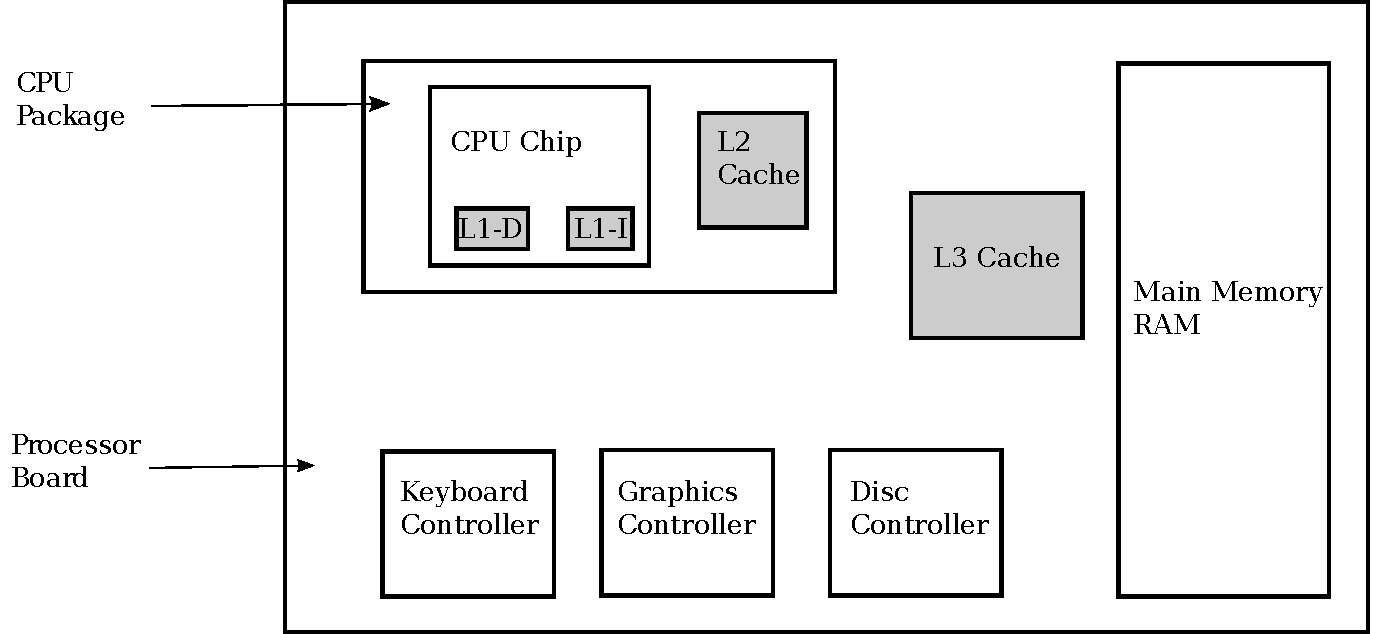
\includegraphics[width=\textwidth]{CacheLevels.pdf}
\caption{The three cache levels}
\label{fig:CacheLevels}
\end{figure}

Figure~\ref{fig:CacheLevels} shows how the three cache are placed in the relation to the CPU. 
The L1 cache resides on the CPU chip itself and usually has a size in the range from 16 KB to 128 KB and because it is placed directly on the CPU chip it is able to provide very fast memory access.
The L2 cache is placed next to the CPU chip on the CPU package and it is connected to the CPU via a high speed path. The L2 cache typically has a size between 512 KB and 1 MB which means that it can hold more data but is not able to provide as fast access as L1.
The L3 cache is placed on the processor board and usually has a size around 3 MB. Since it is placed further away from the cpu it is not able to provide as fast access as L1 and L2 but still much faster than fetching data from RAM.

All three caches are inclusive which means that L2 contains the data from L1 and L3 contains the data from L2.
This means that if data is evicted from L1 it will still reside in the L2 and L3 caches or if data is evicted from L2 it will still reside in L3. 
This is an advantage because it allows fast access to data even if it is evicted from L1 or L2. 
If the caches were not inclusive then it would result in a many more data requests to the main memory which is quite slow in relation to cache data access.

There are two types of address locality that the L1, L2 and L3 caches depends on; Spatial locality and Temporal locality.
Spatial locality occurs when memory locations that has addresses numerically similar to a recently accessed memory location are likely to be requested again very soon.
Temporal locality happens when memory locations that has been accessed recently are accessed again.
The cache exploits spatial locality by fetching more data than has been requested, assuming that it is possible to anticipate future requests.
Temporal locality is exploited by choosing what to evict on a cache miss and normally it is the data entries that has not been accessed recently that are evicted.

Data in the main memory is split into blocks of fixed size called \textit{cache-lines}. 
There are usually 4 to 64 consecutive bytes in a \textit{cache-line}. 
Some of these \textit{cache-lines} are always present in the caches. 
If a requested word is in the cache a trip to main memory can be saved but if the word is not in the cache then a \textit{cache-line} must be removed from the cache and the \textit{cache-line} containing the word must be fetched from main memory or a lower level cache if one is present. 
This is called a \textbf{cache miss} and has a high penalty because fetching a new \textit{cache-line} is expensive.
The general idea is to have the most heavily used \textit{cache-lines} in the caches as often as possible to reduce the amount of cache misses.

\subsubsection{Cache associativity}
When designing a cache it is important to consider whether each \textit{cache-line} can be stored in any cache slot or only in some of them.
There are three approaches to solving this problem; \textit{direct mapped cache}, \textit{n-way set-associative cache} and \textit{fully associative cache}. 
In a \textit{direct mapped cache} each \textit{cache-line} can only be stored in a specific cache slot.
This means that two \textit{cache-lines} cannot be mapped to the same slot simultaneously.
Given a memory address it is only necessary to look for it in one place in the cache and if it is not there then it is not in the cache. Using this approach post consecutive memory lines in consecutive cache slots. 




\subsection{Branch Mispredictions}

\subsection{Translation Lookaside Buffer misses}
